\documentclass[10pt]{article}

\usepackage[margin=0.75in]{geometry}
\usepackage{amsmath,amsthm,amssymb}
\usepackage{xcolor}
\usepackage{cancel}
\usepackage{graphicx}
\usepackage{changepage}
\usepackage{circuitikz}
\usepackage{pgfplots}
\usepackage{physics}
\usepackage{hyperref}
\usepackage{siunitx}
\usepackage{fontspec}
\usepackage{relsize}
\usepackage{subfig}
\usepackage{todonotes}
\usepackage{multicol, multirow, booktabs}
\usepackage[breakable]{tcolorbox}
\usepackage[inline]{enumitem}

\theoremstyle{definition}
\newtheorem{problem}{Problem}
\newtheorem{soln}{Solution}

\pgfplotsset{compat=newest}
\usetikzlibrary{lindenmayersystems}
\usetikzlibrary{arrows}
\usetikzlibrary{calc}
\usetikzlibrary{positioning, fit}
\usetikzlibrary{3d, perspective}

\definecolor{incolor}{HTML}{303F9F}
\definecolor{outcolor}{HTML}{D84315}
\definecolor{cellborder}{HTML}{CFCFCF}
\definecolor{cellbackground}{HTML}{F7F7F7}
\newcommand{\ui}{\hat{i}}
\newcommand{\uj}{\hat{j}}
\newcommand{\uk}{\hat{k}}
\newcommand{\ux}{\hat{x}}
\newcommand{\uy}{\hat{y}}
\newcommand{\uz}{\hat{z}}
\newcommand{\primed}[1]{#1^\prime}
\pgfdeclarelayer{background}  
\pgfsetlayers{background,main}
\AtBeginDocument{\RenewCommandCopy\qty\SI}

\makeatletter
\newcommand{\boxspacing}{\kern\kvtcb@left@rule\kern\kvtcb@boxsep}
\makeatother
\newcommand{\prompt}[4]{
    \ttfamily\llap{{\color{#2}[#3]:\hspace{3pt}#4}}\vspace{-\baselineskip}
}

\newcommand{\thevenin}[2]{
  \begin{center}
    \begin{circuitikz} \draw
      (0,0) -- (2,0) to[battery1, l_=$V_{Th}\eq#1$] (2,2) 
      to[resistor, l_=$R_{Th}\eq#2$] (0,2)
      ;
      \draw [o-] (-.07,2.079);
      \draw [o-] (-.07,0.079);
    \end{circuitikz}
  \end{center}
}

\newcommand{\norton}[2]{
  \begin{center}
    \begin{circuitikz} \draw
      (0,0) -- (3,0) to[american current source, l_=$I_{N}\eq#1$] (3,2) -- (0,2) (2,0)
      to[resistor, l=$R_{N}\eq#2$] (2,2)
      ;
      \draw [o-] (-.07,2.079);
      \draw [o-] (-.07,0.079);
    \end{circuitikz}
  \end{center}
}

\newcommand{\highlight}[1]{\colorbox{yellow}{$\displaystyle #1$}}

\newcommand{\ti}[1]{\widetilde{#1}}

\newfontface{\Kaufmann}{Kaufmann}
\DeclareTextFontCommand{\kf}{\Kaufmann}
\newcommand{\scriptr}{\fontsize{12pt}{12pt}\kf{r}}

\newfontface{\KaufmannB}{Kaufmann Bd BT}
\DeclareTextFontCommand{\kfb}{\KaufmannB}
\newcommand{\bscriptr}{\fontsize{12pt}{12pt}\kfb{r}}

\newcommand{\bv}[1]{\mathbf{#1}}

\title{Physics 3610H: Assignment III}
\author{Jeremy Favro (0805980) \\ Trent University, Peterborough, ON, Canada}
\date{\today}

\begin{document}
\maketitle

% PROBLEM 1
\begin{problem}
Consider a particle in the infinite square well from $0<x<a$. The eigenstates and eigenvalues of the
T.D.S.E for this system are
\begin{align*}
  \psi_n(x) & =\sqrt{\frac{2}{a}}\sin\left(\frac{n\pi x}{a}\right) \\
  E_n       & =\frac{\hbar^2n^2\pi^2}{2ma^2}
\end{align*}
respectively. We also found that these states form an orthonormal set,
$$
  \int_{\mathbb{R}}\psi^*_n(x)\psi_m(x)dx=\delta_{mn}.
$$
Suppose a particle in such a well is in the following state at $t=0$:
$$
  \Psi(x,0)=A(\psi_1(x)+2\psi_2(x))
$$
\begin{enumerate}[label=(\alph*)]
  \item Find $A$ such that $\Psi(x,0)$ is normalized.
  \item Draw $\Psi(x,0)$ as a function of $x$.
  \item Where is the particle most likely to be found at $t = 0$? (Draw arrow(s) on your plot.)
  \item Where is the particle least likely to be found at $t = 0$? (Draw arrow(s) on your plot.)
  \item What is the probability of finding the particle in the left half of the well (i.e. $0 < x < a/2$)
        at $t = 0$?
  \item Find $\Psi(x,t)$.
  \item Show $\Psi(x,t)$ is normalized for all times $t$.
  \item What is the expectation value of $x$?
  \item If you measured the energy of this particle, what values might you get and what is the
        probability that you will get each of these values?
  \item What is the expectation value of the energy?
\end{enumerate}
\end{problem}
\newpage
\begin{soln}~
  \begin{enumerate}[label=(\alph*)]
    \item Here we force the integral over all space of $\abs{\Psi}^2$ to be 1 and solve for an $A$ which satisfies this. We can note
          that because we are dealing with an infinite well here the wavefunction is only nonzero within the well so we can trim down the bounds a bit,
          \begin{align*}
            1 & =\int_{0}^{a}\Psi^*(x,0)\Psi(x,0)\,dx                                                                            \\
              & =\abs{A}^2\int_{0}^{a}(\psi_1^*(x)+2\psi_2^*(x))(\psi_1(x)+2\psi_2(x))\,dx                                       \\
              & =\abs{A}^2\int_{0}^{a}\psi_1^*(x)\psi_1(x)+2\psi_2^*(x)\psi_1(x)+2\psi_2(x)\psi_1^*(x)+4\psi_2(x)\psi_2^*(x)\,dx \\
              & =\abs{A}^2\int_{0}^{a}\psi_1^*(x)\psi_1(x)+2\delta_{12}+2\delta_{12}+4\psi_2(x)\psi_2^*(x)\,dx                   \\
              & =\abs{A}^2\left[\delta_{11}+\cancelto{0}{\delta_{12}+\delta_{12}}+4\delta_{22}\right]                            \\
              & =\abs{A}^2\left[1+4\right]\implies \abs{A}^2=1/5\implies A=\sqrt{1/5}
          \end{align*}
          \todo[inline]{Why doesn't this work for $0<a\leq 3$????}
    \item ~\\
          \begin{center}
            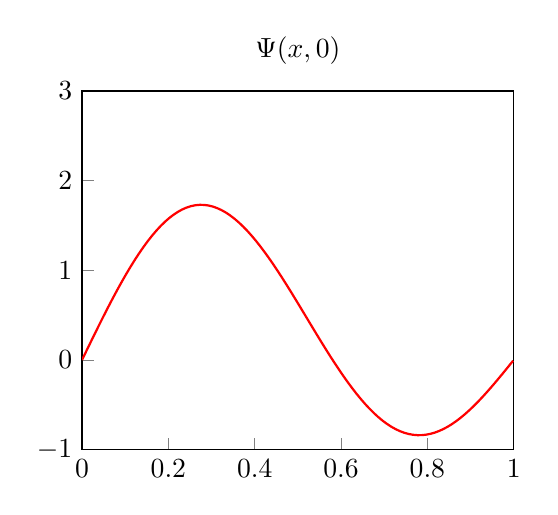
\begin{tikzpicture}
              \begin{axis}[title = {$\Psi(x,0)$},
                  ymax = 3,
                  ymin = -1,
                  xmin=0,
                  xmax=1,
                  xtick pos = bottom,
                  ytick pos = left,
                  scale=0.8]
                \draw[red, thick, domain=0:1, samples=100] plot (\x, {
                    sqrt(1/5)*(sqrt(2)*sin(deg(pi*\x))+2*sqrt(2)*sin(deg(2*pi*\x)))
                  });
              \end{axis}
            \end{tikzpicture}
          \end{center}
    \item Here we take the derivative of the wavefunction $\Psi(x,0)$ and determine the turning points,
          \begin{align*}
            0 & =\frac{d}{dx}\Psi(x,0)                                                                                                                         \\
              & =A\left[\frac{d}{dx}(\psi_1(x)+2\psi_2(x))\right]                                                                                              \\
              & =A\left[\frac{d}{dx}\psi_1(x)+2\frac{d}{dx}\psi_2(x)\right]                                                                                    \\
              & =A\left[\frac{d}{dx}\sqrt{\frac{2}{a}}\sin\left(\frac{\pi x}{a}\right)+2\frac{d}{dx}\sqrt{\frac{2}{a}}\sin\left(\frac{2\pi x}{a}\right)\right] \\
              & =A\sqrt{\frac{2}{a}}\left[\frac{\pi}{a}\cos\left(\frac{\pi x}{a}\right)+\frac{4\pi}{a}\cos\left(\frac{2\pi x}{a}\right)\right] \\
              & =A\frac{\pi}{a}\sqrt{\frac{2}{a}}\left[\cos\left(\frac{\pi x}{a}\right)+4\cos\left(\frac{2\pi x}{a}\right)\right] \\
          \end{align*}
          Which will be zero when 
          $$\cos\left(\frac{\pi x}{a}\right)=-4\cos\left(\frac{2\pi x}{a}\right)$$
          
    \item See blue
    \item What is the probability of finding the particle in the left half of the well (i.e. $0 < x < a/2$)
          at $t = 0$?
    \item Find $\Psi(x,t)$.
    \item Show $\Psi(x,t)$ is normalized for all times $t$.
    \item What is the expectation value of $x$?
    \item If you measured the energy of this particle, what values might you get and what is the
          probability that you will get each of these values?
    \item What is the expectation value of the energy?
  \end{enumerate}
\end{soln}
\end{document}